\documentclass{beamer}

\mode<presentation>
{
  \usetheme{Madrid}       % or try default, Darmstadt, Warsaw, ...
  \usecolortheme{default} % or try albatross, beaver, crane, ...
  \usefonttheme{serif}    % or try default, structurebold, ...
  \setbeamertemplate{navigation symbols}{}
  \setbeamertemplate{caption}[numbered]
} 

\usepackage[english]{babel}
\usepackage[utf8x]{inputenc}
\usepackage{verbatim}
\usepackage{pgfpages}
%\pgfpagesuselayout{resize to}[%
%  physical paper width=8in, physical paper height=6in]

% Here's where the presentation starts, with the info for the title slide

%\title[Chantier Traces: Melty]{Chantier Traces:Melty Data \\ {\small Projet ALGODIV: ANR-15-CE38-001}}
\title[Melty Clustering]{Session Clusterisation : Melty Data \\ {\small Projet ALGODIV: ANR-15-CE38-001}}
%\author[Pedro Ramaciotti-Morales]{Pedro Ramaciotti Morales\\{\tiny pedro.ramaciotti-morales@lip6.fr}}
\institute[LIP6]{LIP6-UMPC, Sorbonne}
\date{\today}
\titlegraphic{
\includegraphics[width=2.5cm]{Logos/logo_algodiv.png}\hspace*{4.00cm}~%
   
\includegraphics[width=1.5cm]{Logos/LIP6_trans.png}
}

\begin{document}

\begin{frame}
  \titlepage
\end{frame}

\begin{frame}{Clustering}
    Clustering on 5 dimensions:
    \begin{enumerate}
        \item requests
        \item timespan
        \item standard\_deviation
        \item inter\_req\_mean\_seconds
        \item read\_pages
    \end{enumerate}
\end{frame}

\begin{frame}{Clustering: 6 clusters}
    \begin{center}
        \resizebox{\textwidth}{!}{
            \begin{tabular}{ccccc}
                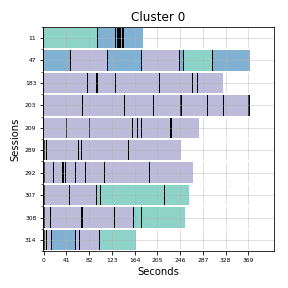
\includegraphics[width=\textwidth, keepaspectratio]{clusters/6/cluster0} & 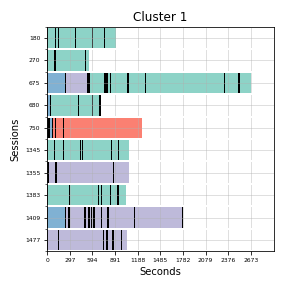
\includegraphics[width=\textwidth, keepaspectratio]{clusters/6/cluster1} & 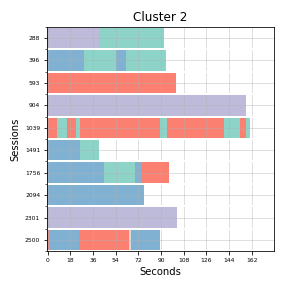
\includegraphics[width=\textwidth, keepaspectratio]{clusters/6/cluster2} & 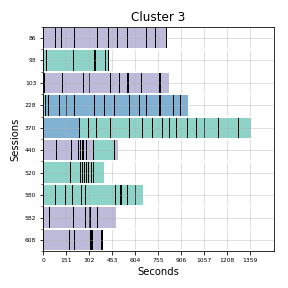
\includegraphics[width=\textwidth, keepaspectratio]{clusters/6/cluster3} & 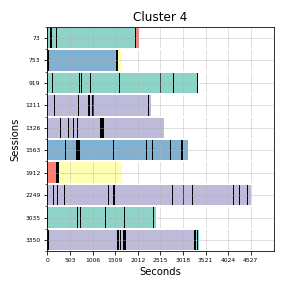
\includegraphics[width=\textwidth, keepaspectratio]{clusters/6/cluster4} \\
                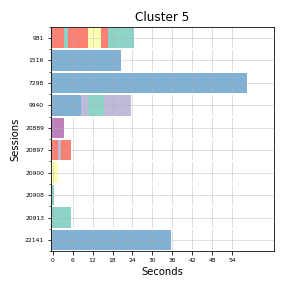
\includegraphics[width=\textwidth, keepaspectratio]{clusters/6/cluster5}
            \end{tabular}
        }

        \begin{columns}
            \begin{column}{.65\textwidth}
                \begin{center}
                \scalebox{.25}{
                    \begin{tabular}{|c|c|c|c|c|c|c|}
                        \hline
                        cluster & size & requests & timespan & standard\_deviation & inter\_req\_mean\_seconds & read\_pages \\
                        \hline
                        0 & 88555 & 0.140 & 0.007 \\
                        \hline
                        1 & 54958 & -0.190 & -0.019 \\
                        \hline
                        2 & 30921 & 0.335 & 0.002 \\
                        \hline
                        3 & 87570 & -0.010 & 0.005 \\
                        \hline
                        4 & 40059 & -0.405 & 0.003 \\
                        \hline
                        5 & 6499 & 0.754 & -0.030 \\
                        \hline
                    \end{tabular}
                }
                \end{center}
            \end{column}
            \begin{column}{.35\textwidth}
                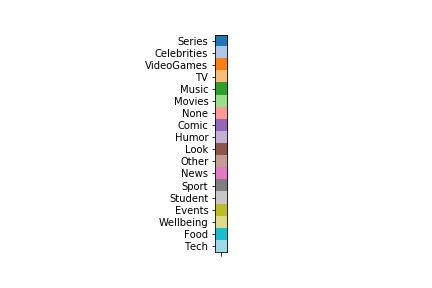
\includegraphics[width=\textwidth, keepaspectratio]{clusters/palette_topic}
            \end{column}
        \end{columns}
    \end{center}
\end{frame}





\end{document}
